%
% Modified by Megan Patnott
% Last Change: Jan 18, 2013
%
%%%%%%%%%%%%%%%%%%%%%%%%%%%%%%%%%%%%%%%%%%%%%%%%%%%%%%%%%%%%%%%%%%%%%%%%
%
% Modified version of the sample_ndthesis.tex
% by Sameer Vijay
% Last Change: Wed Jul 27 2005 14:00 CEST
%
%%%%%%%%%%%%%%%%%%%%%%%%%%%%%%%%%%%%%%%%%%%%%%%%%%%%%%%%%%%%%%%%%%%%%%%%
%
% Sample Notre Dame Thesis/Dissertation
% Using Donald Peterson's ndthesis classfile
%
% Written by Jeff Squyres and Don Peterson
%
% Provided by the Information Technology Committee of
%   the Graduate Student Union
%   http://www.gsu.nd.edu/
%
% Nothing in this document is serious except the format.  :-)
%
%%%%%%%%%%%%%%%%%%%%%%%%%%%%%%%%%%%%%%%%%%%%%%%%%%%%%%%%%%%%%%%%%%%%%%%%
% This is *not* a substitute for the documentation, which is included
% as a pdf file in the standard distribution, and can be obatined from
% the dtx file in the advanced distribution.
%%%%%%%%%%%%%%%%%%%%%%%%%%%%%%%%%%%%%%%%%%%%%%%%%%%%%%%%%%%%%%%%%%%%%%%%
%
% You should *also* have a ND formatting guide to ensure that you have
% all the relevant parts, put the captions in the right place, etc.
% Just because you have this wonderful style classfile doesn't mean
% that it removes *all* the formatting onus from you.  :-)
% Although be warned that the Graduate School has been known to let
% their official formatting guide get out of date. When in doubt,
% the Microsoft Word example seemed to be the only thing kept
% consistently up-to-date in 2013, and is probably the safest thing
% to consult.
%
% You should break all of this stuff up into separate files
% (at the very least, one chapter per file) and use the \include
% command, as has been done here for chapters 1 and 2 and the appendix.
% There is also an \input command, but \include is more commonly used to
% import chapters in books and dissertations. For the differences between these
% two commands, see, e.g., 
% http://web.science.mq.edu.au/~rdale/resources/writingnotes/latexstruct.html
% or http://tex.stackexchange.com/questions/246/when-should-i-use-input-vs-include.
%
% If you compile from the command line, note that you should also have 
% a good Makefile; one that invokes LaTeX as many times as necessary 
% (up to 4) and bibtex if necessary.
%
% If you use an editor that allows you to compile from within the
% program, note that you will need to compile up to four times. Also,
% we recommend that you use pdflatex (sometimes displayed as
% LaTeX => PDF) to compile directly to pdf.
%
% If you have any suggestions, comments, questions, please send e-mail
% to: dteditor@nd.edu
%
%%%%%%%%%%%%%%%%%%%%%%%%%%%%%%%%%%%%%%%%%%%%%%%%%%%%%%%%%%%%%%%%%%%%%%%%

\documentclass[final,numrefs,sort&compress]{nddiss2e}
\usepackage{ mathrsfs }
% One of the options draft, review, final must be chosen.
% One of the options textrefs or numrefs should be chosen
% to specify if you want numerical or ``author-date''
% style citations.
% Other available options are:
% 10pt/11pt/12pt (available with draft only)
% twoadvisors
% noinfo (should be used when you compile the final time
%         for formal submission)
% sort (sorts multiple citations in the order that they're
%       listed in the bibliography)
% compress (compresses numerical citations, e.g. [1,2,3]
%           becomes [1-3]; has no effect when used with
%           the textrefs option)
% sort&compress (sorts and compresses numerical citations;
%           is identical to sort when used with textrefs)

\begin{document}

\frontmatter % All the items before the first chapter go in ``frontmatter''

% Titles may be 1-4 lines long. If your title is longer than 4 lines,
% the class file may have difficulty formatting the title page.
% Line-breaks in the title have to be protected with `\protect`.
\title{Search for lepton flavor violating decays \protect\\ of Higgs Bosons \protect\\ with the CMS experiment}
\author{Nabarun Dev}
\work{Dissertation} % or \work{Thesis}
\degaward{Doctor of Philosophy \\ in \\Physics} % or 
%\degaward{Master of Science \\ in \\ Subject}
\advisor{Colin Philip Jessop}
\department{Physics}

\maketitle
%%%%%%%%%%%%%%%%%%%%%%%%%%%%%%%%%%%%%%%%%%%%%%%%%%%%%%%%%%%%%%%%%%%%%%%%
%
% Front stuff
%
%%%%%%%%%%%%%%%%%%%%%%%%%%%%%%%%%%%%%%%%%%%%%%%%%%%%%%%%%%%%%%%%%%%%%%%%

\makepublicdomain

% An abstract is optional for a mster's thesis, and required for a doctoral dissertation.
\begin{abstract}
  Please note that the full \LaTeX\ source code (and an associated
  \texttt{Makefile}) is available from the University of Notre Dame
  Graduate Student Union web site.  The Information Technology
  Committee page\footnote{\url{http://www.gsu.nd.edu/}}
  has all the necessary files in download-able form.  This particular
  dissertation was developed under Unix, but is also be usable
  under Windows with the appropriate \LaTeX\ setup and was modified
	on a Windows system in 2012-2013. It should also work with on Mac.
  
  While the source code for this document provides an excellent
  example for how to use the \nddiss\ \LaTeX\ class to write a
  Notre Dame thesis, it is \emph{not} a substitution for the
  documentation of the \nddiss\ \LaTeX\ class (also available on
  the ND GSU web site).

  In this thesis, I will tell all that I know about Gnus.  Gnus are
  wonderful little creatures that inhabit the center of the earth and
  give us wonderful and plentiful trees, dirt, and other
  earthly-things.
  
  In short, we should love and cherish the Gnus.  They can be very
  friendly, and are often mistaken for squirrels on the University of
  Notre Dame campus.  Feed them whenever possible.  If they get caught
  in trash cans, tip them over so that they can get out.

  This abstract is going to continue on, including a few formulas,
  just for the sake of spilling over on to two pages so that we can
  see the author's name in the top right corner:
  
	\begin{align*}
    a^2 + b^2 &= c^2 \\
    E &= mc^2 \\
    \frac{e}{m} &= c^2 \\
    a^2 + b^2 &=\frac{e}{m}
  \end{align*}

  These equations, by themselves mean nothing.  But to the common Gnu,
  they define a whole way of living.  While intricate mathematical
  implications certainly do not infiltrate the majority of humans'
  lives, every Gnu, from birth, is imbued with a sense of mathematical
  certainty and guidance.  All Gnus, great and small, feel at one with
  mathematics.  The cute furry bit is just a scam for their
  calculating minds.
\end{abstract}

% A dedication is optional.
\renewcommand{\dedicationname}{Dedicated to}

\begin{dedication}
  To my family
\end{dedication}

% These are required, and must be in this order.
\tableofcontents
\listoffigures
\listoftables

% A preface is optional.
\begin{preface}
  I would like to preface this work with all the wonderful things that
  Gnus have brought to our society: trees, dirt, flowers, grass,
  lakes, and other earthly-things.  We should not forget them in our
  daily lives.

  Additionally, we should offer them food for all their hard work.  In
  fact, Gnus work so hard that they sleep for the colder half of
  the year.  As such, they tend to grow a little rotund.  Humans
  should not fault them for this, as it is necessary for their
  survival.  Indeed, many humans grow rotund on their on accord!
\end{preface}

% It's hard to tell from the information available from the Graduate
% School in Spring 2013 whether or not an acknowledgements section is optional.
\begin{acknowledge}
  I would like to acknowledge all the loving Gnus at Notre Dame.
  Particularly the one that comes to the window in the Hayes Healy
  building.  He (she?) has given me much inspiration, love, and dirt.
  I would also like to thank my advisor, Dr.\ Gary Greenfield, with
  whom this work would not have been possible.

  Finally, I would like to thank the U.S.\ Government, Department of
  Gnus, for their generous grant, number GNU3042920920.3, which
  allowed me to pursue my work.
\end{acknowledge}

% A symbols section is optional.
\begin{symbols}
  \sym{\mathcal{F}}{sighting frequency of Gnus about campus}
  \sym{p}{student population}
  \sym{f}{type of food available}
  \sym{d}{day of week}
  \sym{c}{speed of light}
  \sym{m}{mass}
  \sym{e}{elementary charge}
  \sym{a,b}{miscellaneous constants}  
  \sym{E}{energy}  
\end{symbols}

\mainmatter
% Place the text body here.
%\include{chapter-one}
%Begin each chapter with \chapter{Title}. Both the thesis title and
%chapter titles should match in style.

%
% An unnumbered chapter (features)
%
\unnumchapter{Features of Formatting in This Example File}
% The \unnumchapter command allows you to include an unnumbered chapter as part of
% the main text before Chapter 1. It will appear in your table of contents, and you
% should have at most one such chapter (although nothing in the class file will
% prevent you from creating more).

% The usual \cite{} command is also available, and should work as expected.
This \verb+chapter+ has been added to the original sample file to highlight the
various features with the formatting that conforms to the Graduate school
guidelines --- whether obtained due to the use of \nddiss\/ class file or just
plain good practice.
\begin{itemize}
\item An important note on line-breaks via \verb+\\+ in titles: the
  titles of the thesis as well as chapters and table captions use
  \verb+\MakeTextUppercase{}+ from the \verb+textcase+ package.  Due
  to the nature of the \verb+center+ environment, any line-breaks
  introduced in titles and captions should be protected, as in
  \verb+\protect\\+.
  To preserve the case in titles and captions, use, e.g.,
  \verb+\NoCaseChange{Gnus}+.
\item In the \emph{dedication}, the title name has been modified. So, you know
how to and that it can be done.
\item The entries in the \emph{List of figures} and \emph{List of Tables} are
single-spaced themselves but are double-spaced from the other.
\item The table captions are not in all CAPS as well for the reason mentioned
above.
\item Appropriate space is left between the \verb+Table xx+ and its
corresponding caption (which is double-spaced itself) as in table \ref{tbl:bogus1}.
\item Tables look much better without the vertical lines (good practice).
\item There is double-spacing between the table entries but single-spacing
within the entry.
\item The chapter (see Chapter \ref{chap:golfing}) or section titles are
double-spaced as mentioned in the guidelines.
\item There is a \verb+subsubsection+ present (eg. section \ref{sec:data}) and
is properly formatted in the TOC.
\item Sections deeper than \verb+subsubsection+ should not appear in the TOC.
\item Table \ref{tbl:defs} is an example of the use of \textsf{landscape}
environment in which a normal table is formatted in a \emph{landscape} mode.
\item The \textsf{longtable} environment is used in Tables \ref{tbl:votes} and
\ref{tbl:rotated-rankings}, in normal and \verb+landscape+ mode, respectively. The
table captions are formatted properly in both cases.
\item In the table \ref{tbl:votes}, the \verb+footnote+ in the table header 
does not appear at all. This is not an error of the \nddiss\/ class but of the
\textsf{longtable} package.
\item An example of citing a website is shown in the bibliography (see
\citep{gairley2000}) which is formatted using the \verb+nddiss2e.bst+
citation style file.
\item A bit of information on the \nddiss\/ class file and the typesetting program
used is included in a box on the last page of the thesis.
\item Footnotes should space properly.
\item Items in \verb+itemize+, \verb+enumerate+, and \verb+description+ environment
should automatically single-space within an item, but double space between items.
\end{itemize}

%
% Chapter 1
%

%
% Modified by Megan Patnott
% Last Change: Jan 18, 2013
%
%%%%%%%%%%%%%%%%%%%%%%%%%%%%%%%%%%%%%%%%%%%%%%%%%%%%%%%%%%%%%%%%%%%%%%%%
%
% Modified by Sameer Vijay
% Last Change: Tue Jul 26 2005 13:00 CEST
%
%%%%%%%%%%%%%%%%%%%%%%%%%%%%%%%%%%%%%%%%%%%%%%%%%%%%%%%%%%%%%%%%%%%%%%%%
%
% Sample Notre Dame Thesis/Dissertation
% Using Donald Peterson's ndthesis classfile
%
% Written by Jeff Squyres and Don Peterson
%
% Provided by the Information Technology Committee of
%   the Graduate Student Union
%   http://www.gsu.nd.edu/
%
% Nothing in this document is serious except the format.  :-)
%
% If you have any suggestions, comments, questions, please send e-mail
% to: ndthesis@gsu.nd.edu
%
%%%%%%%%%%%%%%%%%%%%%%%%%%%%%%%%%%%%%%%%%%%%%%%%%%%%%%%%%%%%%%%%%%%%%%%%


%
% Chapter 1
%

\chapter{Introduction}


The standard model of particle physics is the most complete description of nature available today. The discovery of the Higgs Boson added another feather to the hat of the standard model...

...expand...








% % uncomment the following lines,
% if using chapter-wise bibliography
%
% \bibliographystyle{ndnatbib}
% \bibliography{example}



%
% Chapter 2
%

%
% Chapter 2
%

\chapter{Theoretical Background}
\label{chap:theory}
\epigraph{If I have seen further it is by standing on the shoulders of Giants.}{\textit{Isaac Newton}}
\section{Introduction}
In this chapter, we describe the theoretical motivations that drive the searches described in this thesis. We start with a description of the standard model (SM), its particle content and interactions, and the Higgs mechanism. We then talk about the inadequacies of the SM, and the existence of physics beyond the standard model (BSM). We then outline a few BSM models and how they point towards the possible existence of the decays that we search for in this thesis.  

\section{The Standard model }
\label{sec:SM}
The SM is the result of human endeavors over centuries to understand what we and the world around us are made of, and capture those ideas in beautiful mathematical form. Our understanding of the world around us has refined progressively from the ancient times, when best tools of observation we had were nothing but our own eyes, to the current day when we are able to collide particles that make up matter at unprecedented speeds, and have sophisticated tools like the CMS detector to aid us. From the ancient greeks who pondered over philosophical questions about what the basic elements of nature were, to the discovery of electron in 1898 by J.J.Thompson, to Rutherford's famous gold foil experiment, to the discovery of the neutron by James Chadwick in 1932, each event has been a stepping stone towards our understanding of nature and the formulation of SM~\cite{th_gun}. During the course of its formulation and after, the SM has accurately explained phenomena already known and predicted the existence of particles that were discovered later. The last of these particles is the Higgs Boson (h), discovered in 2012 at CERN by the CMS and the ATLAS experiments~\cite{Aad:2012tfa, Chatrchyan:2012ufa, Chatrchyan:2013lba}. The SM is a gauge theory, in which three of the four known natural forces (strong, electromagnetic, weak and not gravity) are represented by the SU(3)$\times$SU(2)$\times$U(1) symmetry group. This symmetry group describes under which transformations the SM is invariant. By Noether's theorem each of the above symmetries associated with the SM Lagrangian is associated with a conserved quantity: color charge, weak isospin and electric charge. The following describes the elementary particles of the SM, the interactions among these and finally, the spontaneous symmetry breaking mechanism.

\subsection{Elementary particles}
There are two kinds of elementary particles in the SM. They are characterized by the intrinsic angular momentum that they carry, i.e. by their spin. Fermions, which have half-integer spins, form the building blocks of matter. Bosons, which have integer spins, are the force-carriers or mediators of interactions.

\subsubsection{Fermions of SM}
\label{fermions}
Fermions we described here are fundamental particles, i.e. they cannot be broken down into further constituents. The space-time evolution of the fermions is described by the Dirac equation and their behavior follows Fermi-Dirac statistics. All fermions are subject to the Pauli exclusion principle. They can be further categorized into two classes depending on their interaction with the strong force. Fermions which do not interact with the strong force are called leptons, and do not carry any color charge. Quarks carry color charge and interact via the strong force. Both leptons and quarks are further classified into three generations. Each lepton generation consists of a lepton and a neutrino while each quark generation consists of a up-type and a down-type quark. These are outlined in detail below.

Leptons comprise of the familiar electron (e), and its heavier cousins -- muon ($\Pgm$) and tau lepton ($\Pgt$), which carry the same negative electric charge as the electron ($1.6\times10^{-19} C$).  The heavier leptons $\Pgt$ ($\sim 1.8\,\mathrm{GeV}/c^2$ ) and $\Pgm$ ($\sim 105.7\,\mathrm{MeV}/c^2$) have short lifetimes of $\sim 2.9\times 10^{-13}\,$s and $\sim 2.2\times 10^{-6}\,$s respectively. They eventually decay into an electron which is the lightest lepton ($\sim 0.5\,\mathrm{MeV}/c^2$ ) and has infinite lifetime, or lighter hadrons. In the CMS detector, the $\mu$ survives long enough to reach the muon systems, and is thus detected as its own distinct signature. The $\Pgt$ on the other hand, owing to its extremely short lifetime, can travel only a very short distance ($\sim <10\,mm$) before decaying. Thus, only decay products of tau leptons are able to be directly detected by CMS. Each charged lepton is associated with an electrically neutral neutrino. They are called electron neutrino ($\nu_e$), muon neutrino ($\nu_{\mu}$) and tau neutrino ($\nu_{\mu}$). Because neutrinos carry no electric charge, they do not interact via electromagnetic interaction. This means the only way they interact is via the weak interaction. This makes neutrinos very difficult to detect. In particular, they pass through the CMS detector effectively without interacting at all, and their presence and the energy they carry can only be estimated using imbalance in transverse momentum of observed particles (see section~\ref{mt_met_recon}). The three generations of leptons are pictorially shown below. 

\begin{equation*}                                                                                                                          
 \binom{e^{-}}{\nu_{e}} \;\;\; \binom{\mu^{-}}{\nu_{\mu}} \;\;\; \binom{\tau^{-}}{\nu_{\tau}}                                           
 \end{equation*}

Quarks come in two generations: up-type and down-type. The up-type quarks are the up quark (u), charm quark (c) and top quark (t). Their down-type counterparts are down quark (d), strange quark (s) and bottom quark (b). Each up-type quark carries a positive electric charge of 2/3 times the charge of the electron. Each down-type quark carries a negative electric charge of 1/3 times the charge of the electron. Just like the leptons, each progressive generation is heavier with the third generation consisting of the top and bottom quarks being the heaviest. In fact, the top quark was the last of the SM fermions to be discovered in 1995, and is the most massive particle in the SM ($\sim 173\,\mathrm{GeV}/c^2$). As mentioned above, all quarks carry color charge. Color charge is to strong force as electric charge is to electromagnetic force. This allows quarks to interact via the strong force. Due to a phenomenon called color confinement, quarks aggregate together into color singlets (having zero color charge) particles called hadrons. Hadrons are either formed of 3 (anti-)\,quarks (baryons) or 2 (anti-)\,quarks (mesons). The proton and neutron are baryons. The proton is made of two up quarks, and one down quark. It has a mass of $\sim 938.3\,\mathrm{MeV}/c^2$ and is stable (infinite lifetime). The neutron is made of one up quark and two down quarks. It has a mass of $\sim 939.5\,\mathrm{MeV}/c^2$ and has a lifetime of $\sim880\,$s. The three generations of quarks are pictorially shown below.

\begin{equation*}
  \binom{u}{d} \;\;\; \binom{c}{s} \;\;\; \binom{t}{b}
\end{equation*}

Each particle described above has an anti-particle associated with it. Particles (matter) and their anti-particles (anti-matter) are almost identical except they have opposite physical charges (electric charge, lepton number, baryon number). For example, the anti-particle of an electron is the positron which is nearly identical to the electron except for the fact that it has positive electric charge.

\subsubsection{Bosons of SM}
The bosons in SM are carriers or mediators of force. Their behavior follows Bose-Einstein statistics and they are not constrained by the Pauli exclusion principle. The strong interaction, as its name suggests, is the strongest of the fundamental forces\,(see table~\ref{tab:forces}). The eight gluons mediate the strong interaction between particles with color charge. Photons are the mediators of the next strongest fundamental force, the electromagnetic force. Gluons and photons are massless, electrically neutral and have spin 1. Additionally, gluons carry color charge. This is in contrast to photons which are electrically neutral. The $\mathrm{W}^+$,$\mathrm{W}^-$ and Z gauge bosons mediate the weak interaction between particles of different flavors. Both bosons have spin 1. However, unlike the photons and the gluons, they are massive. The W boson has a mass of $\sim 80.4\,\mathrm{GeV}/c^2$ and the Z boson has a mass of $\sim 91.2\,\mathrm{GeV}/c^2$. Finally, the Higgs field, the quanta of which is a massive, scalar (spin 0) and electrically neutral Higgs boson, is responsible for giving masses to W, Z bosons and fermions. Table~\ref{tab:forces} shows the relative strength of fundamental forces and their range.         

\begin{table}[hbtp]
\begin{center}
\caption{Relative strengths and ranges of all four fundamental forces, with the strong force as the baseline}
\begin{tabular}{c|c|c}
\hline
Interaction & Relative Strength & Range \\
\hline
Strong & $10^{39}$ & $10^{-15}\,m$\\
Electromagnetic & $10^{36}$& $\infty$\\
Weak &  $10^{24}$ &$10^{-18}\,m$\\
Gravity & $1$ &$\infty$\\
\hline
\end{tabular}
\label{tab:forces}
\end{center}
\end{table}

A pictorial summary of all particles in the SM, divided into different classes is shown in Figure~\ref{fig:sm_zoo}.

\begin{figure}[hbtp]
 \begin{center}
   \includegraphics[width=0.9\textwidth]{plots_and_figures/chapter2/SM_particles.pdf}
   \caption{A pictorial summary of particles in the SM. The Higgs boson is shown in yellow. Gauge bosons are shown in red. Leptons and quarks are shown in green and violet respectively~\cite{sm_zoo}.}
   \label{fig:sm_zoo}
 \end{center}
\end{figure}


\subsection{Theory of interactions in SM}
The SM follows the Lagrangian formalism to describe interaction between the particles. Given the SM is a gauge theory, symmetries of the Lagrangian are central to its understanding~\cite{th_muell}. In a gauge theory, the Lagrangian is invariant under certain (groups of) transformations and each such symmetry is associated with a conservation law (Noether's theorem). The underlying symmetry group that the SM Lagrangian is invariant under is SU(3)$\times$SU(2)$\times$U(1), where the group SU(3) corresponds to the strong interaction while the group SU(2)$\times$U(1) corresponds to the electromagnetic and weak (electroweak) interaction. Each group generator is associated with an underlying vector field, the quanta of which are the gauge bosons (gluons, photons, W and Z) described above. We describe the SM interactions briefly below in order of strength.

\subsubsection{Strong and electroweak interactions}
The theory that describes the strong interaction is called Quantum Chromodynamics (QCD). It is a non-abelian gauge field theory based on SU(3) symmetry. Color charge is the quantity conserved under this symmetry. There are three colors: green (g), red (r) and blue (b). Each color has a corresponding anticolor (negative color). As noted earlier, all quarks and gluons have non-zero color charge. Quarks carry a single color, while each of the eight gluons have a color and anticolor charge. The theory being non-abelian, the generator matrices (Gell-Mann matrices) do not commute. The consequence of this is that gluons (unlike photons) can interact with each other.

The theory that was originally formulated to describe the electromagnetic interaction is called Quantum Electrodynamics (QED). It is a gauge field theory based on U(1) symmetry. Electric charge is the quantity conserved under this symmetry and all particles that interact via electromagnetic interaction need to carry electric charge. Unlike the gluons, the photon (because it is electrically neutral) cannot interact with itself. The weak interaction was initially formulated based on the SU(2) symmetry group, with conserved quantity being the weak isospin. The associated gauge bosons are massive and can be electrically neutral (Z) or charged (W). Quarks of (same) different generations can interact with each other via (Z) W bosons. In the 1960s Glashow, Salam and Weinberg combined the theories describing electromagnetic and weak interactions, after realizing that they were different aspects of the same overarching interaction. This is regarded as electroweak unification, and the electroweak interaction is described by a gauge field theory based on combined SU(2)$\times$U(1) symmetry group. The conserved quantities, weak isospin (T) and electric charge (Q) are related via:
\begin{equation}
  Q = T_{3} + \frac{Y_{W}}{2}
\end{equation}
where $\mathrm{T}_{3}$ is the third component of T and $\mathrm{Y}_{W}$ is a quantum number called the weak hypercharge.

The gauge bosons in this theory are divided into a triplet with two electrically charged and one neutral component (corresponding to Ws and Z), and a singlet with no electric charge (corresponding to the photon). However, in order to maintain gauge invariance of the theory, no mass terms are allowed in the Lagrangian. This would require ALL the gauge bosons (and fermions) to be massless. This is known not to be the case. This broken symmetry (photons being massless and W/Z bosons being massive) is explained by the Higgs mechanism~\cite{Englert:1964et,Higgs:1964ia,Higgs:1964pj,Guralnik:1964eu}, described in the next section.

\subsubsection{The Higgs mechanism}
In order to explain how massive gauge bosons come about, the idea of electroweak spontaneous symmetry breaking (EWSB) is introduced. The phenomenon by which EWSB is utilized to give mass to particles is called the Higgs mechanism. Under this mechanism, a new scalar field, $\phi$, called the Higgs field and an associated potential, V$(\phi)$, is introduced. This is represented as doublet and has four degrees of freedom. Three of these four degrees of freedom correspond to the polarizations of the massive W and Z bosons. In order for the Higgs field to interact with W and Z but the not the photon, symmetry has to be broken. The minimum of the potential, i.e. the vacuum state or ground state must be non-zero for this to happen. The parameters of V$(\phi)$ is so chosen such that it has a Mexican-hat (sombrero) shape, which has infinite degenerate non-zero minima. This non-zero minimum is called the vacuum expectation value (vev), which is measured to be 246\,GeV. The direction of symmetry breaking is such that it gives mass to the Z boson but leaves the photon massless. This breaking of symmetry is called spontaneous because there is no particular reason (that we know of) for this direction to have been picked. Nature just happened to spontaneously pick this direction. The Higgs field gives rise to a new massive scalar particle. This particle is the Higgs boson, and corresponds to the fourth remaining degree of freedom of the scalar doublet mentioned above. The fermions acquire mass via Yukawa interaction with the h. The strength of the Yukawa coupling of the h with fermions is proportional to the fermion masses. To summarize, the Higgs mechanism allows the introduction of a mass term for the gauge bosons without breaking the underlying gauge symmetry of the SM Lagrangian. Addition of this field, gives rise to another massive particle, the interactions with which give masses to gauge bosons and fermions. This massive particle is a scalar boson called the Higgs boson, which was discovered in 2012 at CERN by CMS and ATLAS~\cite{Aad:2012tfa, Chatrchyan:2012ufa, Chatrchyan:2013lba}, almost 50 years after it was first predicted to exist. The most recent measurement of the Higgs mass by CMS, combining data from both run I and run II, is: $125.35\pm0.15$\,GeV~\cite{HIG-19-004}. Before the LHC, experiments at LEP and Tevatron looked for existence of the h. It was the last missing piece of the SM, and its discovery can be thought to have concluded an era in particle physics and led us into a newer equally exciting era.


\subsection{Higgs boson production and decays at the LHC}
There are several different ways the Higgs boson can be produced at the LHC~\cite{th_cec}. The LHC collides protons at high energy, and the production modes of the Higgs boson, in order of cross-section, at the LHC are :

\begin{itemize}
%\setlength%{\linespread}{1.2\baselineskip}  
\item \textbf{Gluon-Gluon Fusion (ggH)}: Since gluons are massless, they do not directly couple to the h. This production mode proceeds via quark loop. The ggH production cross-section at 13 TeV is $\sim48.37\,pb$ at N3LO~\cite{YR4}. 
\item \textbf {Vector Boson Fusion (VBF)}: This production mode has the second largest cross section at the LHC. This mode is characterized by two high-momentum quarks in the final state which hadronize to form jets. The VBF production cross-section at 13 TeV center-of-mass energy is $\sim3.77\,pb$ at NNLO.
\item \textbf {Associated Production}: The third largest h production mode at the LHC involves the production of a virtual $W^*/Z^*$ boson that splits into a real boson W/Z boson and a h. The WH production cross-section is  $\sim1.36\,pb$ and the ZH production production cross-section is $\sim0.87\,pb$, at NNLO level for a center-of-mass energy of 13 TeV at the LHC.
\item \textbf {ttH Production}:   In this production mode, the h is produced along with a pair of top quarks. The production cross-section at 13 TeV center-of-mass energy is $\sim0.50\,pb$ at NLO.
\end{itemize}
  
The Feynman diagrams for h production modes described above are shown in Figure~\ref{fig:higs_feyn}. The cross-section of each process as a function of center-of-mass energy is shown in Figure~\ref{fig:higs_xs_som}. Figure~\ref{fig:higs_decays} shows the branching fractions of various SM decays of Higgs boson as a function of its mass, illustrating how branching fractions depend on the Higgs mass. It is interesting to note that the 2012 discovery was made combining the channels where the Higgs decays into Z$\mathrm{Z}^*$, or into $\gamma\gamma$ (di-photon). Even though the Higgs doesn't directly interact with the massless photon, there are loop order contributions. Although, the cross-section of this channel is small compared to the others, its clean final state signature made it one of the primary channels for the discovery.    


\begin{figure}[hbtp]
 \begin{center}
   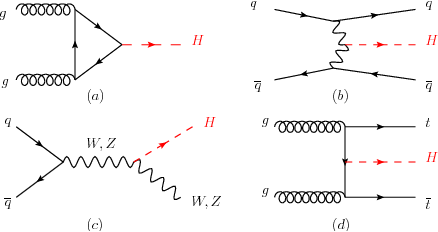
\includegraphics[width=0.95\textwidth]{plots_and_figures/chapter2/higgs_prod.png}
   \caption{ Feynman diagrams for Higgs production modes at LHC: (a) gluon-gluon fusion, (b) vector boson fusion, (c) associated production and (d) ttH~\cite{higg_prod}, are shown.}
   \label{fig:higs_feyn}
 \end{center}
\end{figure}


\begin{figure}[hbtp]
  \begin{center}
    \captionsetup{width=.8\textwidth}
   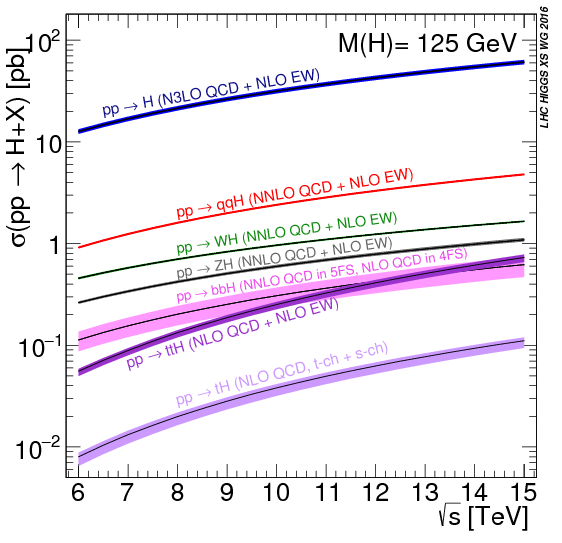
\includegraphics[width=0.9\textwidth]{plots_and_figures/chapter2/higgs_xs.png}
   \caption{The SM Higgs boson production cross-section as a function of the center-of-mass energy in proton-proton collisions at the LHC~\cite{higg_prod}.}
   \label{fig:higs_xs_som}
 \end{center}
\end{figure}
    
\begin{figure}[hbtp]
  \begin{center}
    \captionsetup{width=.8\textwidth}
   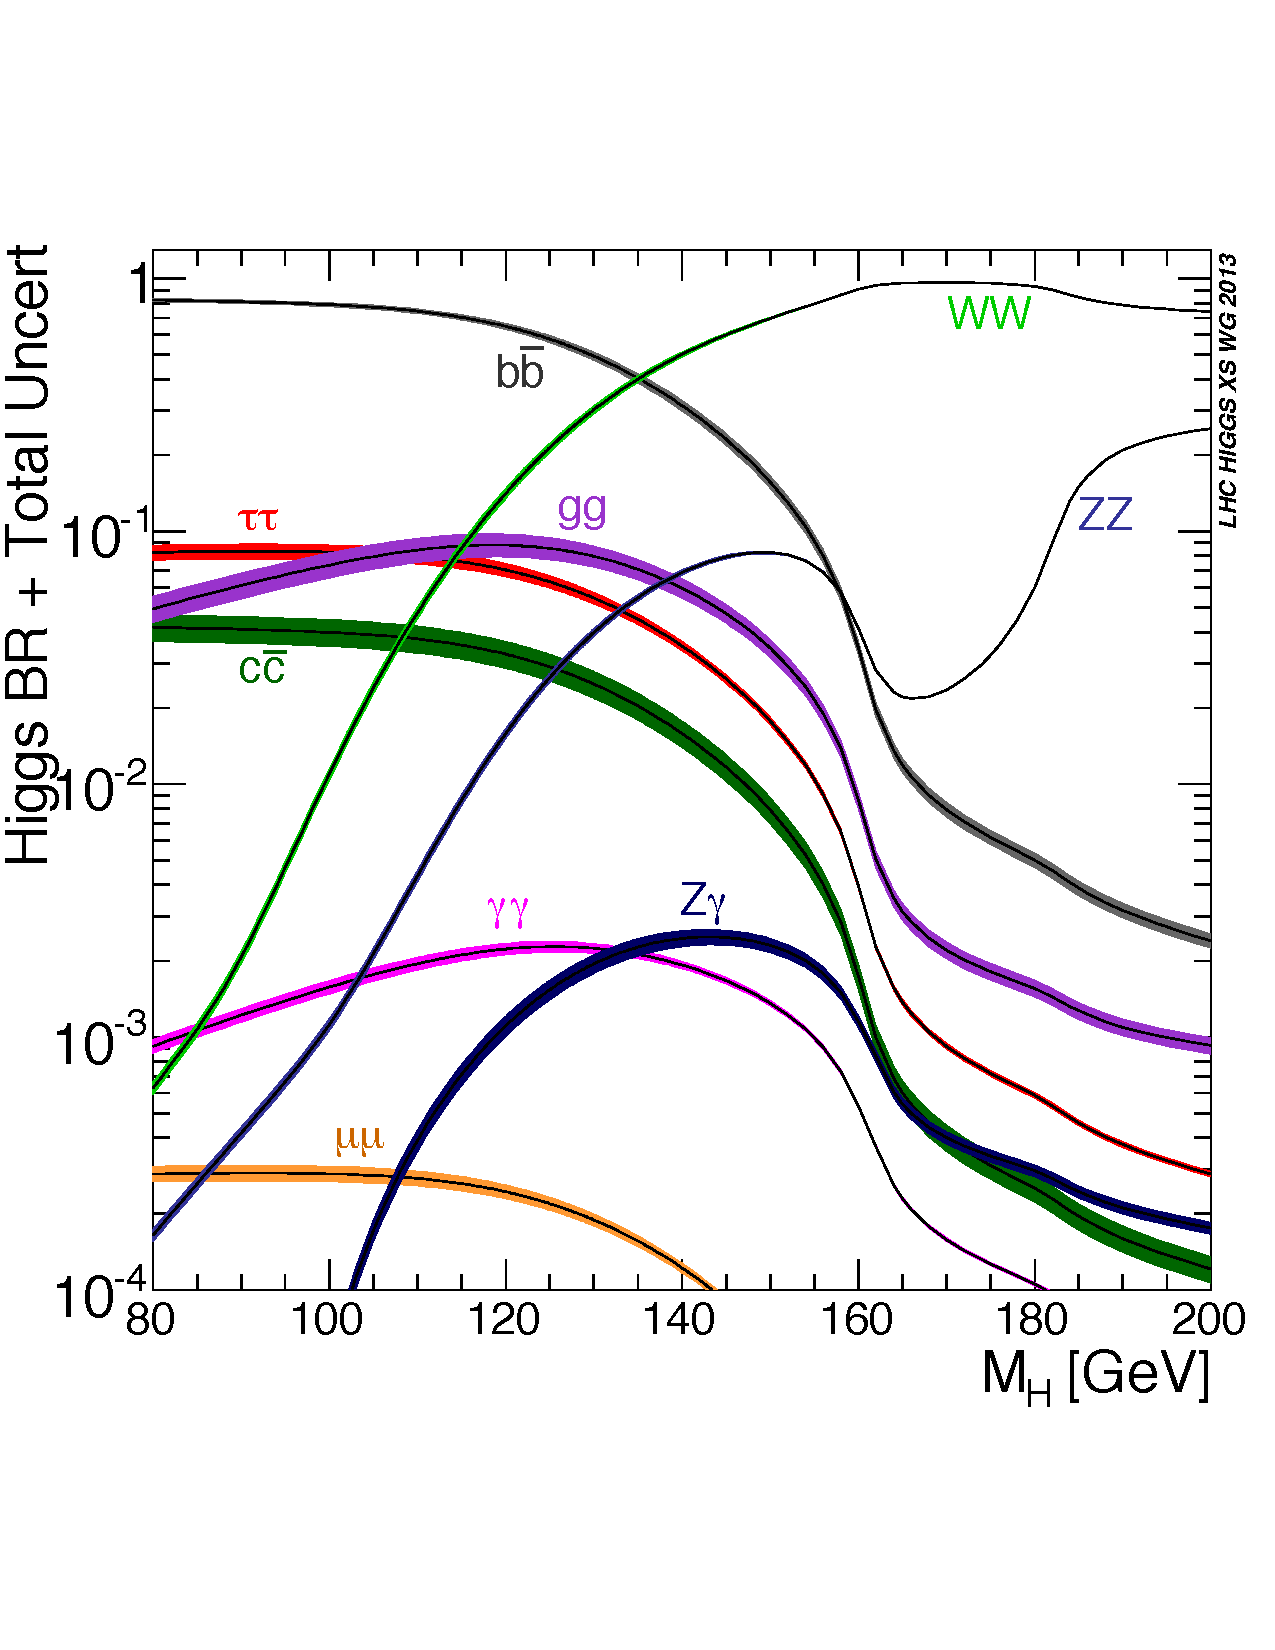
\includegraphics[width=0.9\textwidth]{plots_and_figures/chapter2/higgs_decays.pdf}
   \caption{Branching fractions to SM decays of the Higgs boson as function of mass~\cite{hg_decay}.}
   \label{fig:higs_decays}
 \end{center}
\end{figure}

\section{Inadequacies of the SM}
Despite being a faithful description of nature, the SM is not perfect. There are several motivations that suggest the existence of physics beyond the SM. We outline some of these here.

To start, the SM falls short of being an ideal theory of everything, because it doesn't include gravitation. Including gravitational interaction into the SM has proven to be a difficult challenge. It hasn't yet been possible to incorporate the most successful theory of gravity, General Relativity, and the SM into a single framework. Secondly, neutrinos which are electrically neutral leptons (see section ~\ref{fermions}) are strictly massless within the SM. However, it has been well-established by experiments that neutrinos oscillate (change flavor). This is only possible if neutrinos have mass. The small but finite masses that neutrinos are now known to have doesn't fit with the SM formulation. Thirdly, cosmological observations point to the existence of a type of matter and energy, the origin of which cannot be explained within the SM. They are referred to as dark matter and dark energy. About 26\% of the universe is known to be made of dark matter and 69\% is known to be made of dark energy. Thus, particles of the SM form only 5\% of the observable universe. Finally, it is believed that matter and anti-matter were produced in almost equal amounts at the Big Bang. However, the universe is made almost entirely of matter. There is no mechanism in the SM that explains how we ended up with a matter dominated universe. Besides the unexplained phenomena outlined above, our understanding of some theoretical features of the SM is inadequate. The SM contains no less than 19 numerical free parameters. The values of these parameters are known but we do not have an understanding of their origins.

To address such shortcomings, many theories have been proposed that modify the SM in such a way that they are consistent with existing observations, but at the same time try to address its imperfections. These theories, called BSM (beyond the standard model) theories predict many outcomes that are otherwise not allowed by the SM. The recently discovered h unlocks a portal to look for these outcomes. As mentioned earlier, the constraint on the branching fraction to non-SM decay modes of the h, derived from a combined study by CMS and ATLAS is B(non-SM) $<$ 34\% at 95\% confidence level (CL)~\cite{JHEP2016:45}. These limits suggest a significant contribution from exotic (non-SM) decays in the BSM Higgs sector. One such interesting process that is forbidden in the SM but occurs in many new physics scenarios is interactions between charged leptons that violate the conservation of Lepton Flavor. In particular, Lepton Flavor Violating (LFV) decays of the h are allowed by these theories, and could be realized in decays of the h, which is neutral, into two charged leptons of different flavor. Looking for LFV decays of charged leptons is also interesting in the light of neutrino oscillations mentioned earlier, which also violate lepton flavor, a phenomenon that remains unexplained by the SM~\cite{th_kell}.


\section{BSM models with lepton flavor violation}
\label{sec:BSM}
Like all fermions, charged leptons acquire mass from their interaction with the Higgs. Higgs interacts with these leptons via Yukawa couplings. The Yukawa interaction matrix is diagonal in SM:

\[
  Y=\begin{pmatrix}
    Y_{ee}       & 0 & 0  \\
    0       & Y_{\mu\mu} & 0  \\
    0       & 0 & Y_{\Pgt\Pgt}
  \end{pmatrix}
\]

However, in BSM models, the above doesn't hold true~\cite{Harnik:2012pb} and off-diagonal Yukawa couplings are possible. In a model containing only the SM Higgs as the source of EWSB, an effective field theory approach can be used to introduce off-diagonal couplings~\cite{DiazCruz:1999xe}. If only SM particles (quarks, leptons, gauge and Higgs bosons) are considered to exist up to a certain energy scale, $\Lambda$, additional heavy fields can be integrated out, leading to an effective field theory. Higher dimensional operators of dimension 6 then suffice to introduce LFV couplings. Interestingly, dimension 5 operators introduce neutrino oscillations into the SM, but not LFV in interactions of charged leptons. Dimension 6 operators decouple the values of fermion couplings to the h from the fermion masses. The Yukawa couplings can be then written as:
\begin{equation}
  Y_{ij}=\frac{m_{ij}}{v}\delta_{ij}+\frac{v^2}{\sqrt{2}\Lambda^2}\hat{\lambda}_{ij}
\end{equation}
where $\hat{\lambda}_{ij}$s are coefficients associated with dimension 6 operators. In the limit $\Lambda\rightarrow\infty$, we recover the SM and off-diagonal couplings are zero. Thus, LFV couplings can be introduced as long as the mass scale is finite.  In BSM models with several sources of EWSB, LFV couplings can be introduced without this restriction. Two Higgs doublet models (2HDM) models constitute general models of this class, and allow the violation of lepton flavor~\cite{PhysRevLett.38.622}. Supersymmetry models~\cite{Han:2000jz,Arganda:2004bz,Arhrib:2012ax,Arana-Catania:2013xma,Arganda:2015uca,Arganda:2015naa}, such as the Minimal Supersymmetric Standard model (MSSM) and the Next-to-Minimal Supersymmetric Standard model (NMSSM), also postulate multiple Higgs bosons, and give rise to LFV interactions. Supersymmetric models introduce a alternate (supersymmetric) boson partner to every SM fermion and an alternate fermion partner for every SM boson. These alternate particles, if discovered, could be suitable candidates for explaining dark matter and dark energy. Other models that allow LFV interactions include~\cite{HIG-17-001} composite Higgs models~\cite{Agashe:2009di,Azatov:2009na} which consider the SM h to be a bound state of other BSM particles, partially composite Higgs models such as Randall-Sundrum models~\cite{Perez:2008ee,Casagrande:2008hr,Buras:2009ka}, and several others~\cite{Blanke:2008zb,Giudice:2008uua,AguilarSaavedra:2009mx,Albrecht:2009xr,Goudelis:2011un,McKeen:2012av,Pilaftsis199268,PhysRevD.47.1080,Arganda:2014dta,Ishimori:2010au}.

\section{Pre-LHC constraints on LFV couplings}

Indirect low-energy measurements from pre-LHC era can be used to constrain the $\hmu$ decay. These constraints were derived and summarized in~\cite{Harnik:2012pb}. For example, constraints on $\Pgt\rightarrow\Pgm\gamma$ transition which proceed via a virtual Higgs boson can be used to constrain $\hmu$ decay. Feynman diagrams contributing to this process at one loop level are shown in Figure~\ref{fig:prelhclfv}. Further constraints come from $\Pgt\rightarrow 3\Pgm$ decays, and also from anomalous magnetic dipole moments, and are shown in the same figure. The constraints on Yukawa couplings derived from the above measurements can be converted to constraints on $Br(\hmu)$, following the procedure described in Section~\ref{results}. These constraints set the upper limit on $Br(\hmu)\lesssim 10\%$, thus leaving a lot of room to search for this decay. Similar constraints exist for $\he$ LFV decay, and are set at $Br(\he)\lesssim 10\%$. Indeed, CMS searches looking for $\he$ decay have been performed along with searches for $\hmu$. Finally, it is interesting to note the LFV decay, $\hflep$, is very strongly constrained by $\Pgm\rightarrow\Pe\gamma$ decays, giving an very stringent upper limit $Br(\hflep)\lesssim 2\times10^{-8}$. Due to such strong existing constraints, this search is not been performed by CMS, but rather $\hmu$ (this thesis) and $\he$ searches are performed.           

\begin{figure}[hbtp]
 \begin{center}
   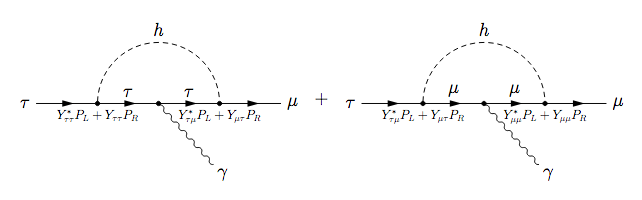
\includegraphics[width=0.9\textwidth]{plots_and_figures/chapter2/tau_mugamma.png}\\
   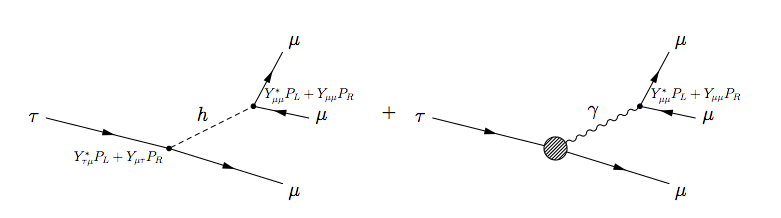
\includegraphics[width=0.9\textwidth]{plots_and_figures/chapter2/tau_3mu.png}\\
   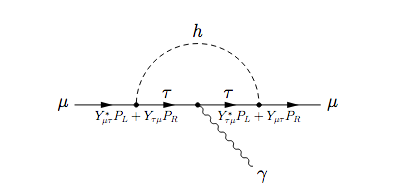
\includegraphics[width=0.6\textwidth]{plots_and_figures/chapter2/dipole.png}
   \caption{Diagrams contributing to flavor violating process $\Pgt\rightarrow\Pgm\gamma$ (top), $\Pgt\rightarrow 3\Pgm$ (middle) and anomalous magnetic moment of the muon (bottom)~\cite{Harnik:2012pb}.}
   \label{fig:prelhclfv}
 \end{center}
\end{figure}

\section{Constraints from previous LHC searches}

The first direct search for LFV Higgs decays was published by CMS collaboration in 2015~\cite{Khachatryan:2015kon}. This search improved the limits listed above by an order of magnitude to $\mathcal{B}(\hmu)<1.51\%$ (0.75\%) for observed (expected) limits at 95\% CL. This was followed by another search (2016) which set observed (expected) upper limits on the branching fractions  $\mathcal{B}(\he)<0.69\%$ (0.75\%) at 95\% CL~\cite{HIG-14-040}. Both searches were performed with 19.7\,$\mathrm{fb}^{-1}$ of pp collision data collected at 8 TeV center-of-mass energy by CMS during Run I of LHC . The limits from these searches are summarized graphically in Figure~\ref{fig:8tev_limits}. In 2015 and 2017, the ATLAS Collaboration also published results from similar searches performed with data collected by the atlas detector~\cite{Aad:2016blu,Aad:2015gha}. The observed (expected) limits were set at $\mathcal{B}(\hmu)<1.43\%$ (1.01\%) and $\mathcal{B}(\he)<1.04\%$ (1.21\%) at 95\% CL.

\begin{figure*}[hbtp]
  \begin{center}
   \captionsetup{width=.7\textwidth,justification=centering}
   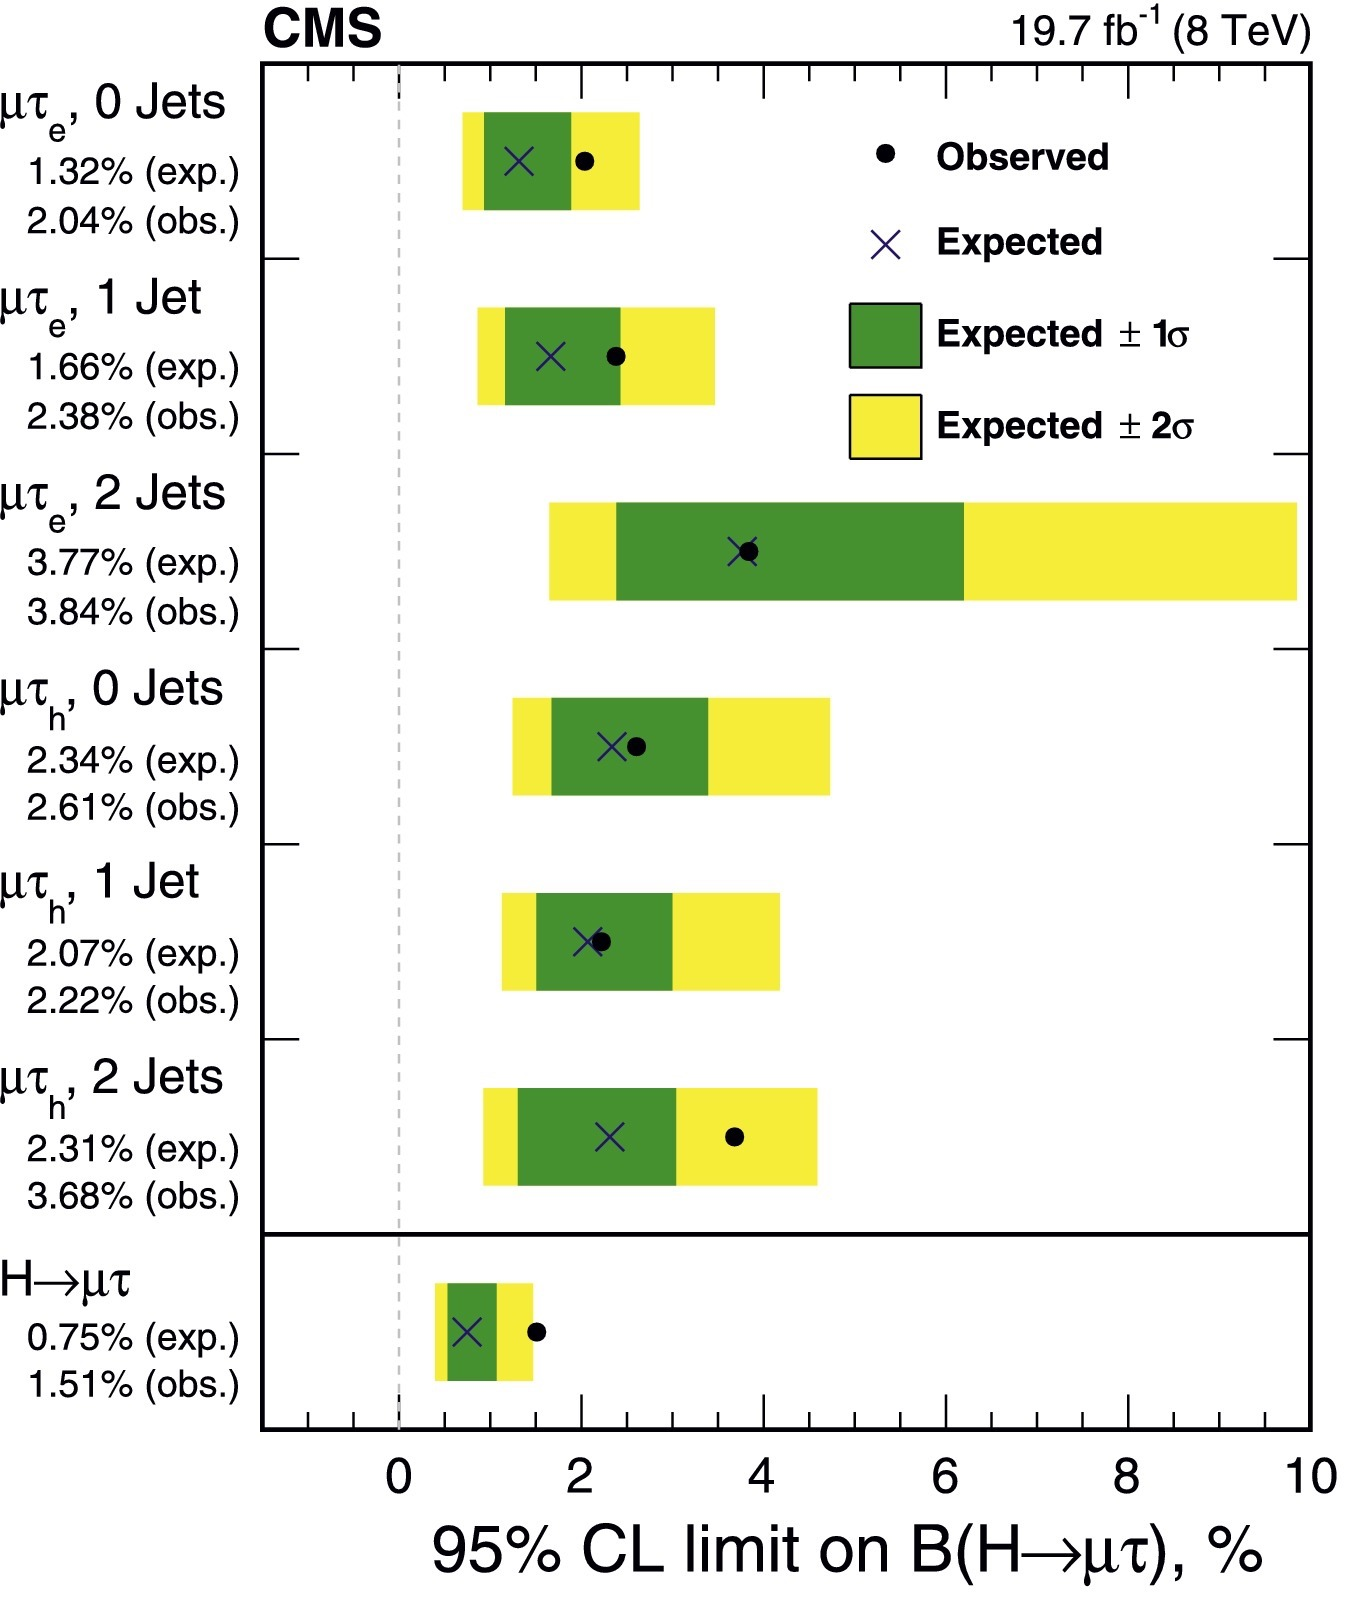
\includegraphics[width=0.6\textwidth]{plots_and_figures/chapter2/mutau_limits.jpg}\\
   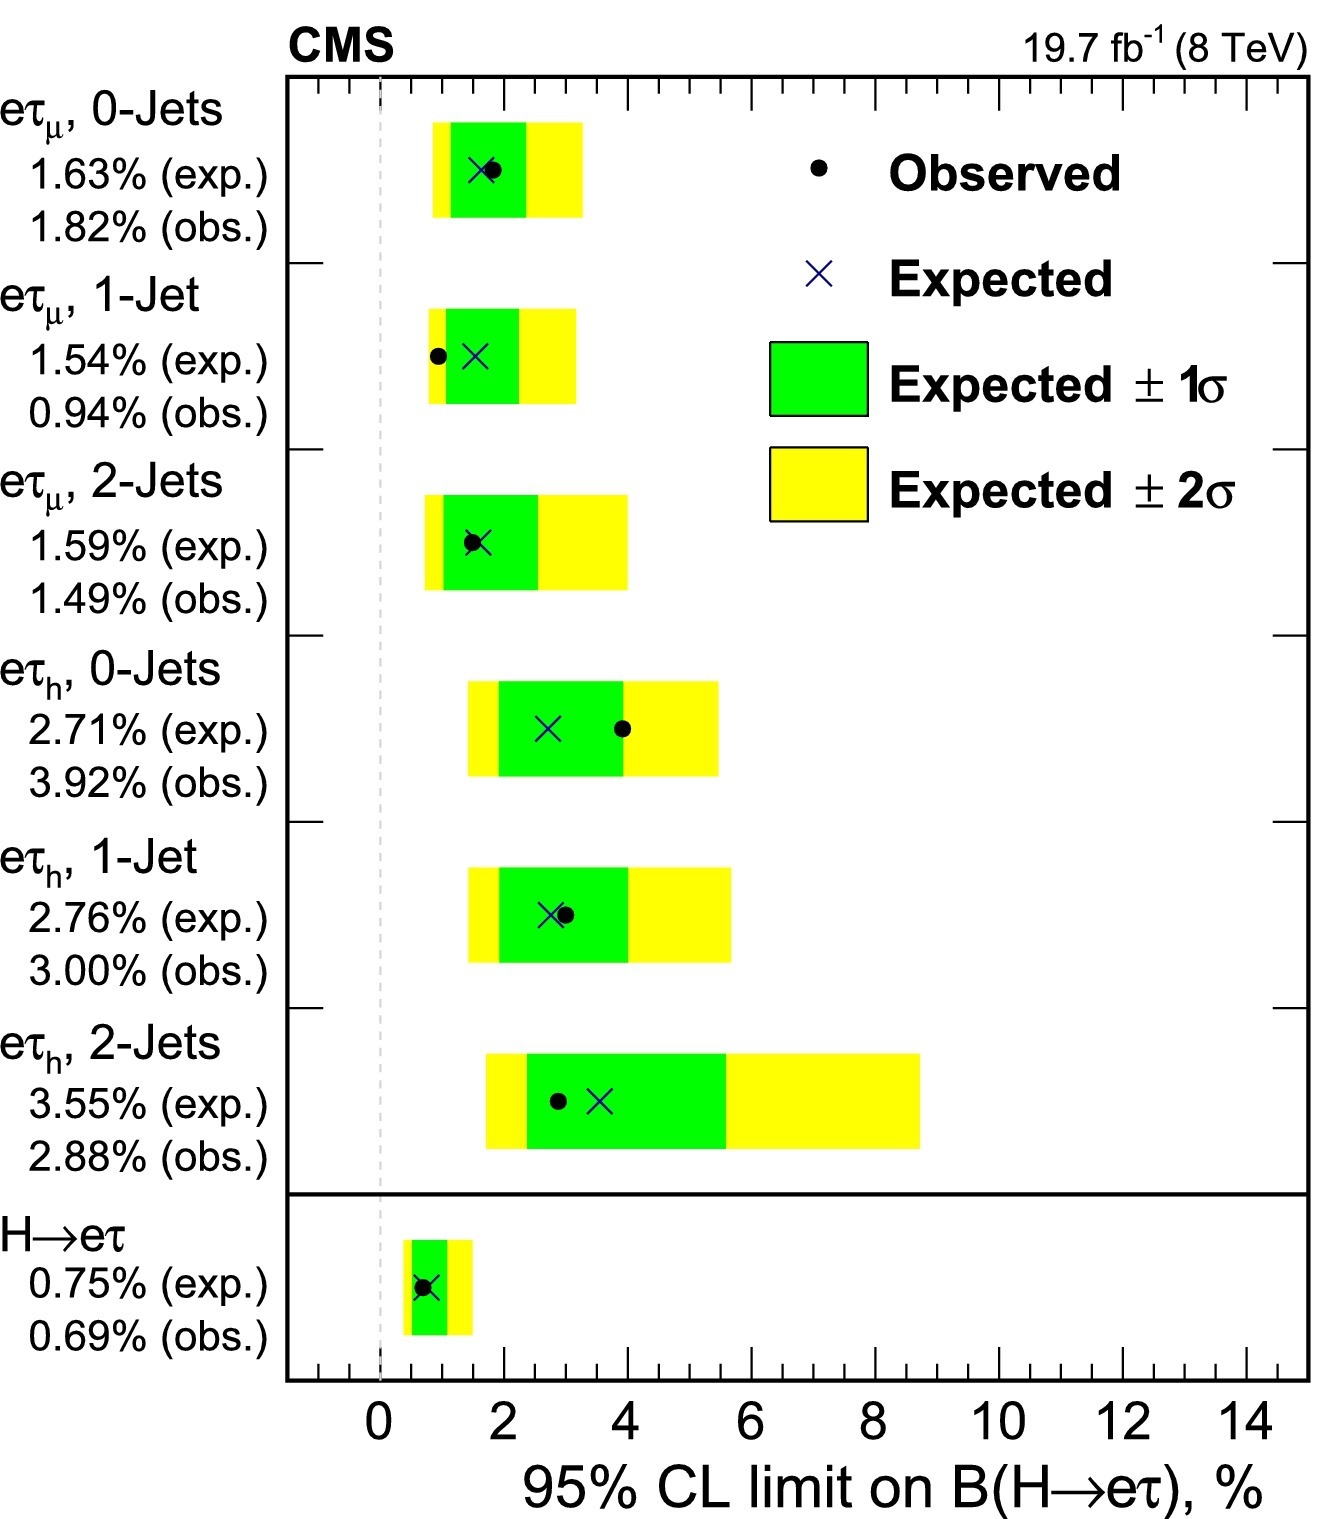
\includegraphics[width=0.6\textwidth]{plots_and_figures/chapter2/etau_limits.jpg}
   \caption{Limits from Run I searches performed by CMS for $\hmu$ (top) and $\he$ (bottom)~\cite{Khachatryan:2015kon,HIG-14-040}.}
   \label{fig:8tev_limits}
 \end{center}
\end{figure*}


The 2015 CMS search for $\hmu$ saw an excess of events with a significance of 2.4\,$\sigma$. Although this excess is not quite enough to claim evidence for this decay, this gives us a strong motivation to perform this search with a larger amount of data which would either lead us to confirm this excess, or squash it and set much stricter limits on this process. The dataset collected by the CMS detector in 2016 provides us with such an opportunity. It corresponds to proton-proton collision data at a much higher center-of-mass energy of 13\,TeV. The number of h bosons produced depends on the cross-section. Since the cross section scales up at higher center-of-mass energies (see Figure~\ref{fig:higs_xs_som}), a much larger number of h bosons would be produced. Also, the 2016 dataset has a size of 36\,$\mathrm{fb}^{-1}$ which is almost two times in size of the run I dataset. This thesis describes this search specifically in the channel where the $\Pgt$ decays into a electron, i.e. the $\hmue$ channel.   

\section{Motivations for $\Hmue$ search}
As mentioned in section~\ref{sec:BSM}, many of the BSM models, that allow LFV decays of the h, predict the existence additional heavy Higgs bosons. For example, 2HDM predicts the existence of two heavy neutral Higgs bosons, H(CP-even) and A(CP-odd). According to a theoretical study published in 2016~\cite{PhysRevD.93.055021}, these heavy bosons (henceforth referred to as H) are expected to decay in a Lepton Flavor Violating manner just like their SM counterpart, h . A direct search for $\Hmu$ would thus provide a complementary probe of these BSM models that postulate the existence of such heavy neutral H bosons. In fact, the 2015 CMS search for $\hmu$ was reinterpreted as a search for $\Hmu$ decay~\cite{Buschmann:2016pb}, and limits on $\sigma(\textrm{gg}\rightarrow \PH)\times\mathcal{B}(\Hmu)$ were set for H bosons in the mass range of 150\,GeV to 300\,GeV. We describe here the first direct search to look for $\Hmu$ decay, in the channel where the $\Pgt$ decays into an electron, i.e. $\Hmue$ channel. Only the primary H production mode (gluon fusion) is considered for this search. This search uses the same dataset as the $\hmu$ search, i.e. 36\,$\mathrm{fb}^{-1}$ of pp collision data at 13 TeV center-of-mass energy collected in 2016, and probes H masses in the range range $200<m_H<900$\,GeV. 



%
% Chapter 3
%

%
% Modified by Megan Patnott
% Last Change: Jan 18, 2013
%
%%%%%%%%%%%%%%%%%%%%%%%%%%%%%%%%%%%%%%%%%%%%%%%%%%%%%%%%%%%%%%%%%%%%%%%%
%
% Modified by Sameer Vijay
% Last Change: Wed Jul 27 2005 13:00 CEST
%
%%%%%%%%%%%%%%%%%%%%%%%%%%%%%%%%%%%%%%%%%%%%%%%%%%%%%%%%%%%%%%%%%%%%%%%%
%
% Sample Notre Dame Thesis/Dissertation
% Using Donald Peterson's ndthesis classfile
%
% Written by Jeff Squyres and Don Peterson
%
% Provided by the Information Technology Committee of
%   the Graduate Student Union
%   http://www.gsu.nd.edu/
%
% Nothing in this document is serious except the format.  :-)
%
% If you have any suggestions, comments, questions, please send e-mail
% to: ndthesis@gsu.nd.edu
%
%%%%%%%%%%%%%%%%%%%%%%%%%%%%%%%%%%%%%%%%%%%%%%%%%%%%%%%%%%%%%%%%%%%%%%%%

%
% Chapter 2
%

\chapter{Experimental Setup}
\label{chap:exper_setup}
..intoduce...
\section{The Large Hadron Collider}
\label{sec:LHC}

The Large Hadron Collider (LHC) is a powerful proton-proton synchrotron. It was built and is operated at the European Center for Nuclear Research (CERN) and is situated about 100 m underground close to Geneva, Switzerland. It has a circumference of 26.7 km and uses a tunnel previously built for LEP (Large Electron Positron Collider). Being a particle-particle collider, it consists of two rings with counterrotating beams which are steered using magnets and accelerated using radiofrequency resonating cavities. These beams are made to intersect at four collision points around the LHC ring, at one of which rests the CMS detector. Besides proton-proton collisions the LHC can also collide heavy ions (lead-lead collisions) or heavy ions with protons (lead-proton collisions). Since starting operation in September 2008 the LHC has been the world's most powerful apparatus and will probably remain so in the forseeable future. The following section describes proton-proton collisions at the LHC as the data used in the subsequent physics analysis corresponds to events from these collisions.

The injector chain that supplies protons to the LHC consists of four CERN accelerators that actually predate the LHC: Linac 2, PSB (Proton Synchroton Booster), PS (Proton Synchotron) and SPS (Super Proton Synchotron). This is illustrated in figure~\ref{fig:cern_acc_comp}. The proton source is simply tank of hydrogen gas. The hydrogen atoms are ionized to yield protons which are then fed in the Linac 2, a linear accelerator. This accelerates the protons to an energy of about 50 MeV which are then fed into a series of circular accelerators starting with the PSB which accelerates the protons to 1.4 GeV. The PS then accelerates them to 25 GeV and they are then sent to the SPS which accelerates them to 450 GeV before being finally fed into the LHC beampipe. Inside the LHC the protons are accelerated by sixteen radiofrequency cavities which are made to oscillate at 400 MHz and the proton beam is sorted into discrete packet called 'bunches'. The beam is steered by 1232 Niobium-Titanium superconducting dipole magnets and collimated using quadrupole magnets. This magnet system is kept at a temperature below 2 K, using a pressurised bath of superfluid helium at about 0.13 MPa, and operates at fields above 8T. The LHC has three sophisticated vacuum systems: the insulation vacuum for cryomagnets, the insulation vacuum for  helium  distribution, and the beam vacuum.

\begin{figure*}
\begin{center}
\includegraphics[width=0.8\textwidth,keepaspectratio]{plots_and_figures/cern_acc_complex.png}
\caption{Cern Accelerator Complex}
\label{fig:cern_acc_comp}
\end{center}
\end{figure*}


It takes about 4 minutes and 20 seconds to fill up the each of the LHC rings wih protons, and about 20 minutes for the proton beam to reach its current peak energy 6.5 TeV. At this point, each LHC beam contains 2808 bunches each consisting of $1.5 \times 10^{11}$ protons, and colliding at a center of mass energy of 13 TeV. It is anticipated for the COM energy to increase to 14 TeV in 2018. Looking for physics beyond the standard model by colliding protons at such high energies is one of the primary aims of the LHC.

Another important parameter for a collider like the LHC is the instantaneous luminosity, \mathscr{L}.




So why do gnus do what they do?  This is a perennial question that has
yet to be answered definitively by scientists.  Is their future
somehow tied inexplicably with that of humans?  Hard to say, but we do
feed them a lot.  It has even been theorized that rotundness is a
symbol of status or class within the Gnus; those who are more
productive (i.e., cute, furry, friendly) will be fed more than those
who are less so.  So the more rotund, the higher status one has in the
Gnu society.

One could extrapolate this to mean that there is a super-Gnu out there
somewhere; the biggest, rotundest Gnu that you've ever seen, probably
of epic proportions!  This would have to be the Leader of Gnus, or LoG
for short.  But the LoG would definitely have to be the cutest,
furriest, and most friendly Gnu that you've ever seen.

\subsection{The LoG}

So how does the LoG get chosen?  Ultimately by humans.  So we can say
that the Gnu society is perhaps the truest democracy that has ever
existed; the leader is chosen by merit, and chosen by complete
outsiders.  As such, the LoG must truly epitomize all that Gnus stand
for: opposedness to overmanagement, cuteness, friendliness, and
furriness~\citep{gloonson98:_gnuly_discov_gnus}.  The gnus themselves
vote at an anual election, based upon these attributes (campagaining
is an anethema to Gnus; see Section~\ref{sec:groovin-gnus}).

\section{Physics beyond the standard model}
\label{sec:BSM}

Table~\ref{tbl:votes} shows the latest electoral college voting by the
LoG for the year 2000.  Each Gnu is scored on a scale of one to ten on
the attributes described above.  The results shown in the table are
average scores in each category for all votes; the Gnu's final score
is shown in the final column.

%
% Be aware that page-spanning tables a Very Odd Creatures.  The
% "longtable" environment in LaTeX does some deep Voodoo to make
% everything work out properly.  One of its deep incantations is to
% make the table appear as though it is double spaced.  You can fix
% this by trailing each line with "\\[-6em]" instead of just "\\".
% When using longtable it is also important to compile your file
% more than once. But you're probably already doing this to get
% the internal references correct, anyway.
%

\begin{center}
  \begin{longtable}{lccccc}
    \caption{Electoral College Results for the \NoCaseChange{LoG} Election in the Year
2000\label{tbl:votes}\/}\\
        \toprule
        Candidate\footnote{note all names begin with G} & Anti-management & Cuteness & Friendliness & Furriness & Aggregate \\
        \midrule
\endfirsthead % Everything above goes at the top of the 1st page only
% As with the first header, we don't want obscene amounts of space for
% subsequent headings either, and eliminate an em of whitespace.
  \caption[]{{\em Continued}}\\
  \midrule
  Candidate & Anti-management & Cuteness & Friendliness & Furriness & Aggregate \\
  \midrule
\endhead % Everything above here (and below the \endfirsthead) goes at the top
         % of continuation pages.  The [] argument prevents a duplicate
         % entry from appearing in the table of contents.
% The following 3 lines are provided as an example only -- per ND
% guidelines, the footer at the bottom of a page for a longtable
% should not have a bottom line.  Only the absolute bottom of the
% table should have a final \bottomline

%  \midline
%  \multicolumn{6}{|r|}{\textit{continued}\ldots} \\
%  \bottomrule
\endfoot % The above section goes at the bottom of continuation pages
  \bottomrule
\endlastfoot % The very last bottom of the table
    Glen & 6.2 & 7.0 & 6.1 & 9.8 & 7.2 \\
    Goober & 6.9 & 2.1 & 5.7 & 4.1 & 4.6 \\
    Genevra & 2.2 & 2.0 & 1.1 & 1.1 & 1.6 \\
    Greg & 8.3 & 0.4 & 1.1 & 9.5 & 4.8 \\
    Gina & 6.0 & 7.8 & 6.4 & 4.9 & 6.2 \\
    Geof & 1.1 & 8.7 & 3.7 & 7.3 & 5.2 \\
    Grendel & 2.8 & 1.7 & 3.4 & 3.2 & 2.7 \\
    Geronimo & 1.2 & 1.2 & 8.8 & 2.2 & 3.3 \\
    Gabrielle & 4.7 & 3.6 & 0.8 & 2.0 & 2.7 \\
    Giovani & 8.4 & 5.8 & 3.4 & 7.4 & 6.2 \\
    Graham & 4.7 & 5.8 & 5.3 & 0 & 3.9 \\
    Gil & 5.9 & 4.0 & 5.5 & 7.6 & 5.7 \\
    Gerald & 2.0 & 3.7 & 8.0 & 4.3 & 4.5 \\
    Guilani & 7.7 & 3.9 & 2.7 & 6.4 & 5.1 \\
    Guido & 7.6 & 4.3 & 6.5 & 1.0 & 4.8 \\
    Godzilla & 5.1 & 2.2 & 5.3 & 6.9 & 4.8 \\
    Gail & 5.7 & 7.9 & 4.1 & 1.0 & 4.6 \\
    Garth & 4.7 & 7.1 & 2.5 & 3.0 & 4.3 \\
    Gavin & 1.1 & 9.5 & 0.4 & 8.0 & 4.7 \\
    George & 9.5 & 4.5 & 9.1 & 7.5 & 7.6 \\
    Gunnar & 1.4 & 5.8 & 4.8 & 6.2 & 4.5 \\
    Gillian & 7.6 & 9.0 & 6.4 & 4.6 & 6.9 \\
    Greta & 1.5 & 0.5 & 0.9 & 7.7 & 2.6 \\
    Gabby & 1.2 & 3.3 & 7.0 & 2.1 & 3.4 \\
    Gaetena & 6.8 & 1.9 & 4.1 & 8.3 & 5.2 \\
    Ganet & 2.3 & 1.1 & 8.5 & 7.3 & 4.8 \\
    Gardenia & 1.8 & 9.5 & 9.9 & 3.0 & 6.0 \\
    Genna & 5.2 & 3.7 & 3.4 & 3.8 & 4.0 \\
    Genesis & 1.7 & 8.3 & 6.7 & 4.9 & 5.4 \\
    Genaveve & 4.7 & 8.9 & 3.4 & 9.2 & 6.5 \\
    Gene & 3.3 & 6.9 & 0.6 & 5.5 & 4.0 \\
    Gilda & 5.2 & 4.6 & 9.9 & 1.4 & 5.2 \\
    Goldie & 8.9 & 9.1 & 2.0 & 8.2 & 7.0 \\
    Grace & 5.9 & 3.2 & 3.1 & 4.3 & 4.1 \\
    Gretchen & 4.5 & 6.5 & 1.6 & 1.3 & 3.4 \\
    Garrick & 4.8 & 5.7 & 9.4 & 5.1 & 6.2 \\
    Gallagher & 7.4 & 0.4 & 7.6 & 0.4 & 3.9 \\
    Gerry & 1.4 & 8.8 & 4.7 & 0.5 & 3.8 \\
    Gertrude & 9.1 & 8.3 & 0.4 & 5.5 & 5.8 \\
    Gehosephet & 6.6 & 2.9 & 8.3 & 4.4 & 5.5 \\
    Gohn & 8.7 & 2.6 & 7.4 & 2.3 & 5.2 \\
    Gibby & 8.7 & 6.9 & 4.7 & 7.2 & 6.9 \\
  \end{longtable}
\end{center}

As you can see from Table~\ref{tbl:votes}, George (my favorite Gnu)
won for the year 2000, with an aggregate score of 7.6.

% % uncomment the following lines,
% if using chapter-wise bibliography
%
% \bibliographystyle{ndnatbib}
% \bibliography{example}



%
% Appendix (optional)
%

\appendix

%
% Modified by Sameer Vijay
% Last Change: Wed Jul 27 2005 13:00 CEST
%
%%%%%%%%%%%%%%%%%%%%%%%%%%%%%%%%%%%%%%%%%%%%%%%%%%%%%%%%%%%%%%%%%%%%%%%%
%
% Sample Notre Dame Thesis/Dissertation
% Using Donald Peterson's ndthesis classfile
%
% Written by Jeff Squyres and Don Peterson
%
% Provided by the Information Technology Committee of
%   the Graduate Student Union
%   http://www.gsu.nd.edu/
%
% Nothing in this document is serious except the format.  :-)
%
% If you have any suggestions, comments, questions, please send e-mail
% to: ndthesis@gsu.nd.edu
%
%%%%%%%%%%%%%%%%%%%%%%%%%%%%%%%%%%%%%%%%%%%%%%%%%%%%%%%%%%%%%%%%%%%%%%%%

%%%%%%%%%%%%%%%%%%%%%%%%%%%%%%%%%%%%%%%%%%%%%%%%%%%%%%%%%%%%%%%%%%%%%%%%
%
% Appendix
%
%%%%%%%%%%%%%%%%%%%%%%%%%%%%%%%%%%%%%%%%%%%%%%%%%%%%%%%%%%%%%%%%%%%%%%%%

\chapter{GNU GENERALISMS}

\section{Definitions}

Several definitions are presented in Table~\ref{tbl:defs} to show both
how to do rotated, line-spanning tables, as well as to define some
commonly used Gnu terms.

\begin{landscape}
\begin{table}
\centering
\caption{Commonly used \NoCaseChange{Gnu} Terms \label{tbl:defs}}
\begin{tabular}{lp{5in}}
\toprule
Term & \multicolumn{1}{c}{Definition} \\
\midrule
Gnu & Small furry animal that is related to the squirrel 
(although they won't admit it). \\
LoG & Abbreviation for the ``Leader of Gnus''.  See
Chapter~\ref{chap:golfing}. \\
Twizzlers & Red, twisty candy that is among the most favorite of Gnu
foods.  Gnus frequently appear overly cute and friendly to humans
bearing twizzler packages.  This is known as ``trolling for twizzlers''
among the Gnus. \\
\bottomrule
\end{tabular}
\end{table}
\end{landscape}

Finally, Table~\ref{tbl:rotated-rankings} shows the top ten Gnus from
Table~\ref{tbl:votes} ranked in order by their aggregate score (along
with some of the raters' comments).  This follows a long-standing Gnu
tradition of self-improvement through public announcement of score
(which some associate with military
origins~\citep{galmira98:_gnus_milit}).  Indeed, this very table has
been observed in the Gnu lodge where it was posted for peer review
\citep{gairley2000}.


\begin{landscape}
% set the caption width to be somewhat short since our table is narrow
% Notice the special commands that we use here to get the right line in the
% table.  Using \hrule is *not* the Right Thing to do here -- use
% \cmidrule.  We use the LaTeX \newcommand simply for convenience.
%
% The longtable package does some nasty voodoo to make \hline work OK.
% So on with the goods
\setlength\LTcapwidth{4.5in}
\begin{longtable}{lcp{4.5in}}
% Note that after the caption line we remove 2em worth of space but in the
% longtable of Chapter 2 we only remove 1em.  This is because a normal 
% \toprule has no space above it, but here we are using cmidrule which does 
% have padding above which we must account for.
  \caption{Top Ten \NoCaseChange{Gnus} From
    Table~\NoCaseChange{\ref{tbl:votes}} With Reviewer Comments.
    \NoCaseChange{Gnus} are Listed Below in Alphabetic Order.
    \label{tbl:rotated-rankings} }\\
  \toprule
  Candidate & Aggregate score & \multicolumn{1}{c}{Reviewer Comments}\\
  \midrule
\endfirsthead
  \caption[]{{\em Continued}} \\  % Just like in Chp. 2
  \midrule
  Candidate & Aggregate score & \multicolumn{1}{c}{Reviewer Comments}\\
  \midrule
\endhead
\endfoot
  \bottomrule
\endlastfoot
George & 7.6 & George is an excellent candidate for the LoG.
  Slightly low C, but hopefully, this 7.6 will be high enough! \\
Glen & 7.2 & A little weak on AM and Fr, but good scores overall.  One
  or two more years of experience should be enough. \\
Goldie & 7.0 & Dismal score in Fr; suspect it had something to do with
  strenuous weight loss program this past year. \\
Gillian & 6.9 & Excellent C, but a little shabby on the Fu.  Suggest
  more roughage. \\
Gibby & 6.9 & Reasonable scores, but need to work on Fr.  Gibby is
  definitely not a morning Gnu. \\ 
Genaveve & 6.5 & Very low Fr; perhaps more coffee?  Suggest practicing
  ``cute faces'' in the mirror several hours per day.  \\
Giovani & 6.2 & Very low Fr; suspect hanging out with Genaveve too
  much. \\
Gina & 6.2 & Mediochre Fu, somewhat low AM.  Perhaps a future in
  marketing or advertising? \\
Garrick & 6.2 & Fairly low AM.  Fu could be better as well; buy a
  comb.  And a mirror.  Immediately.  \\
Gardenia & 6.0 & Dismal AM; very low Fu.  Seems to care more about
  meeting agendas than personal appearance. \\
\end{longtable}
\end{landscape}


% % uncomment the following lines,
% if using chapter-wise bibliography
%
% \bibliographystyle{ndnatbib}
% \bibliography{example}



%
% Back stuff
%

% % comment out the following three lines
% if using chapter-wise bibliography

 \backmatter
 \bibliographystyle{abbrvnat} % The standard abbrvnat style should be acceptable. Also provided with both the advanced and standard
 \bibliography{example}       % distributions are nddiss2e and nddiss2enoarticletitles style options.
% If you prefer to manually enter your bibliography, that is fine. Comment out the previous two lines, and enter your bibliography
% as usual. Note that if you choose this route, formatting the bibliography is your responsibility. An example is below, including the
% optional arguments necessary for author-date style citations.
%	\begin{thebibliography}{9}
%		\bibitem[Galmira(1998)]{galmira98:_gnus_milit} G.\ Galmira. Gnus and the military -- a secret conspiracy? \emph{Growing Towards Gnu}, III(7):22--183, September 1998.
%		
%		\bibitem[Ganston and Greenfield(1998)]{gnus98:_gerry_ganst} G.\ Ganston and G.\ Greenfield. \emph{Gnus and You: The Art of Being New}. volume I. Grapping Books, NY, August, 1998.
%		
%		\bibitem[Gloonston(1998)]{gloonston98:_gnuly_discov_gnus} G.\ Gloonston. Newly discovered gnus: The LoG. \emph{Growing Towards Gnu}, II(12):23---57, March 1998.
%		
%		\bibitem[Greenfield(1996)]{greenfield96:_gettin_know_gnu} G.\ Greenfield. \emph{Getting to Know Gnu}. PhD thesis, Geoffrey Garfield School of Gnus, August 1996.
%		
%		\bibitem[van Gairley(2000)]{gairley2000} G.\ van Gairley. Gnu's review. Website, 2000. \url{http://www.gairley.gnu}.
%	\end{thebibliography}

\end{document}

% End of ``example.tex''
